\section{Hybridisation Reactions}

Hybridisation reactions are central to the operation cycle of the DNA nanopiston. By
providing the required free energy, they facilitate the transitions between the two
stable states of the cycle, rotaxane-ss and rotaxane-ds. Combining these transitions with
the previously discussed entropic interactions a ratcheting mechanism enables the
extraction of useful work from the inherently stochastic system.\\

The associated length and time scales of these reactions make their in-depth analysis
experimentally challenging. For this reason scientists resort to computational
simulations for high resolution analyses of these reactions. To study the DNA
hybridisation occurring during the piston operation cycle, we utilised our OxDNA based
model of the
piston which is simulated using molecular dynamics. As previously discussed in chapter
three, the intrinsic energy landscape associated with these reactions complicates brute
force simulations of the transitions. To overcome these limitations a forward flux
sampling
algorithm was employed. Illustrating the viability of this technique, first both the
hybridisation and the toehold displacement reactions of the rotaxanes were simulated
outside of the nanopore. From these simulations it was confirmed, that using the forward
flux sampling algorithm the full ensemble of transition path ways present in the
hybridisation reactions can be studied.\\

However, performing these same simulations with the rotaxanes placed inside of the
nanopore inhibited the reaction from occurring. During the final stages of both the
toehold displacement and hybridisation reaction, the geometry of the rotaxane forces
three ssDNA strands inside of the pore's constriction. The diameter of the pore was
modelled to carefully capture both the electrostatic and excluded volume interactions
between the ClyA pore and the DNA, resulting in a diameter of $2.9\ mm$, compared to the
$1\ nm$ width of the ssDNA strand. Due to the static nature of our coarse-grained pore
model, the diameter of the pore constriction does not facilitate the three ssDNA strand
to enter the constriction simultaneously.\\

In literature we find an indication that the $\alpha$-helices constituting the pore's
constriction allow for a reasonable amount of structural fluctuations of the
constriction.\cite{willems2021} Our simulations indicate that the compliancy of the pore
entrance is essential in the hybridisation reaction of the rotaxanes, but where not taken
into account in our model. This limitation of our coarse-grained model impedes the full
analysis of the DNA nanopiston's operating cycle. Improving upon this model by including
the compliance of the pore's constriction was attempted, but did not succeed within the
time constraints of this thesis.

% \begin{figure}[ht!]
%   \centering
%   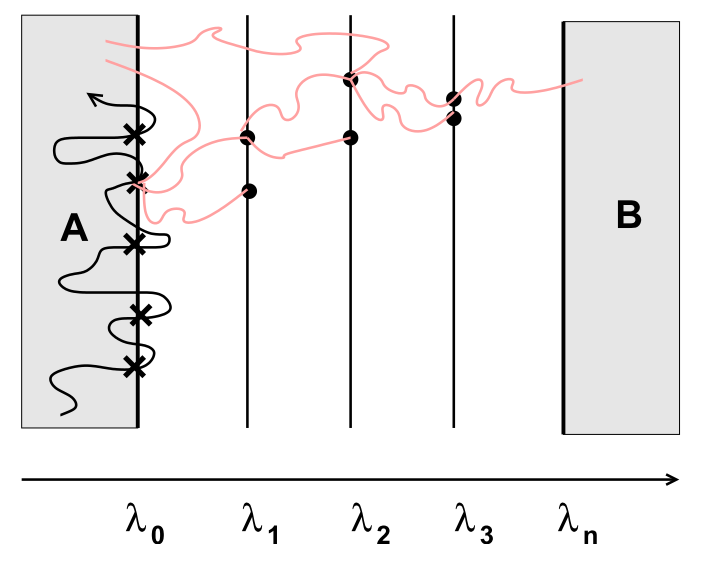
\includegraphics[width=0.6\linewidth]{Figures/FFS.jpg}
%   \caption{Nog maken}
% \end{figure}

